\section{Material and Methods}
\label{sec:material_methods}

\subsection{Theoretical background}
\label{sec:theoretical_background}
El an{\'a}lisis de la movilidad urbana depende cada vez m{\'a}s de sistemas autom{\'a}ticos de percepci{\'o}n capaces de describir las condiciones del tr{\'a}fico a nivel de cada usuario vial. En los sistemas inteligentes de transporte, la vigilancia visual proporciona evidencia sobre presencia, clase, posici{\'o}n, movimiento e interacci{\'o}n de los veh{\'i}culos con la infraestructura vial, y permite abordar tareas de percepci{\'o}n como detecci{\'o}n, clasificaci{\'o}n, estimaci{\'o}n de par{\'a}metros y an{\'a}lisis de comportamiento \cite{Zhou2025TrafficSurveillanceSurvey}. Esta informaci{\'o}n es especialmente importante en intersecciones, donde los flujos heterog{\'e}neos, los giros, las oclusiones y los patrones breves de congesti{\'o}n hacen que la observaci{\'o}n manual sea dif{\'i}cil de escalar. En consecuencia, la fundamentaci{\'o}n te{\'o}rica del estudio parte de la percepci{\'o}n de escenas de tr{\'a}fico y avanza hacia la detecci{\'o}n de objetos con localizaci{\'o}n orientada.

El reconocimiento de im{\'a}genes y la detecci{\'o}n de objetos son tareas relacionadas, pero no equivalentes: el primero asigna una o m{\'a}s etiquetas sem{\'a}nticas a una imagen completa, mientras que la segunda localiza cada instancia y le asigna una clase dentro de la escena visual. Esta diferencia es central en aplicaciones de tr{\'a}fico, porque un solo fotograma puede contener varios veh{\'i}culos de distintas categor{\'i}as, tama{\~n}os y orientaciones. El aprendizaje profundo se ha convertido en el paradigma dominante para la detecci{\'o}n de objetos, ya que las arquitecturas convolucionales y basadas en transformadores pueden aprender representaciones visuales jer{\'a}rquicas directamente desde los datos; dentro de este marco, los detectores contempor{\'a}neos suelen organizarse como enfoques de una etapa o de dos etapas seg{\'u}n la forma en que integran localizaci{\'o}n y clasificaci{\'o}n \cite{Zou2023ObjectDetectionSurvey}. En este trabajo, la tarea te{\'o}rica relevante no es solo reconocer que existen veh{\'i}culos, sino estimar una detecci{\'o}n estructurada para cada instancia visible en cada fotograma.

La detecci{\'o}n vehicular en escenas de tr{\'a}fico y en vistas de tipo a{\'e}reo presenta dificultades espec{\'i}ficas que no siempre aparecen con la misma intensidad en los conjuntos gen{\'e}ricos de detecci{\'o}n. Los veh{\'i}culos pueden aparecer a diferentes escalas debido a la perspectiva de la c{\'a}mara, su posici{\'o}n en la v{\'i}a, la distancia al sensor y la resoluci{\'o}n del fotograma; adem{\'a}s, pueden estar parcialmente ocluidos por otros veh{\'i}culos, infraestructura vial, sombras o desenfoque por movimiento \cite{Ding2022DOTA}. En escenas densas, los objetos cercanos pueden solaparse espacialmente, aumentando el riesgo de localizaciones imprecisas, detecciones duplicadas u omisiones. Las claves contextuales, como la geometr{\'i}a de los carriles, la posici{\'o}n relativa entre veh{\'i}culos y la presencia de otros participantes del tr{\'a}fico, pueden ayudar a resolver casos ambiguos cuando la apariencia del objeto es insuficiente \cite{Jamali2025ContextObjectDetection}. Por estas razones, los sistemas de detecci{\'o}n orientados al tr{\'a}fico requieren modelos y protocolos de evaluaci{\'o}n que consideren variaci{\'o}n de escala, oclusi{\'o}n y contexto de escena.

La detecci{\'o}n de objetos peque{\~n}os es un componente cr{\'i}tico de la detecci{\'o}n vehicular en fotogramas urbanos. Un veh{\'i}culo puede convertirse en un objeto peque{\~n}o cuando ocupa pocos p{\'i}xeles, lo que ocurre con veh{\'i}culos lejanos, motocicletas, mototaxis o instancias ubicadas cerca de los bordes de la escena. Estos objetos son dif{\'i}ciles de detectar porque las operaciones de reducci{\'o}n espacial dentro de las redes profundas pueden debilitar sus caracter{\'i}sticas antes de llegar a las capas de predicci{\'o}n, y porque su apariencia puede contaminarse con p{\'i}xeles del fondo, objetos vecinos o artefactos de compresi{\'o}n \cite{Nikouei2025SmallObjectSurvey}. Para im{\'a}genes de alta resoluci{\'o}n, las estrategias de particionado o \textit{slicing} permiten procesar regiones locales sin reducir excesivamente el tama{\~n}o aparente de los objetos, lo que ha mostrado mejoras en escenarios con objetos peque{\~n}os o lejanos \cite{Akyon2022SAHI}. Este problema es directamente relevante para clases vehiculares compactas y potencialmente subrepresentadas.

La detecci{\'o}n tradicional de objetos representa la localizaci{\'o}n mediante cajas horizontales o \textit{horizontal bounding boxes} (HBB), que son rect{\'a}ngulos alineados con los ejes de la imagen. Esta representaci{\'o}n es simple y eficiente, pero se vuelve imprecisa cuando los objetos aparecen rotados respecto al sistema de coordenadas de la imagen \cite{Wang2025OBBSurvey}. En escenas capturadas desde c{\'a}maras elevadas, oblicuas o ubicadas en intersecciones, los veh{\'i}culos pueden presentar orientaciones arbitrarias debido a giros, carriles diagonales y trayectorias no alineadas con los ejes de la imagen. Las cajas orientadas u \textit{oriented bounding boxes} (OBB) ampl{\'i}an la representaci{\'o}n de localizaci{\'o}n al incorporar un par{\'a}metro angular, permitiendo cubrir de forma m{\'a}s ajustada un objeto rotado y reducir la inclusi{\'o}n de fondo o el solapamiento artificial entre instancias cercanas. Por ello, la detecci{\'o}n con OBB es m{\'a}s adecuada que la detecci{\'o}n con HBB para tareas en las que las instancias aparecen con orientaciones arbitrarias.

Los m{\'e}todos de aprendizaje profundo para detecci{\'o}n orientada se basan en los principios generales de la detecci{\'o}n de objetos, pero incorporan mecanismos adicionales para manejar rotaci{\'o}n, alineamiento y regresi{\'o}n angular. Algunos enfoques buscan alinear las caracter{\'i}sticas convolucionales con anclas o propuestas rotadas, de modo que las caracter{\'i}sticas usadas para clasificar coincidan mejor con la geometr{\'i}a del objeto orientado; S2A-Net aborda esta inconsistencia mediante refinamiento de anclas y alineamiento de caracter{\'i}sticas antes de la predicci{\'o}n orientada \cite{Han2022S2ANet}. Otros modelos incorporan equivarianza rotacional para representar de forma m{\'a}s directa la orientaci{\'o}n de los objetos en im{\'a}genes a{\'e}reas \cite{Han2021ReDet}. Adem{\'a}s, las p{\'e}rdidas de regresi{\'o}n para cajas rotadas pueden formularse mediante distribuciones gaussianas y divergencias, como la divergencia de Kullback-Leibler, para mejorar la precisi{\'o}n de localizaci{\'o}n en objetos con orientaci{\'o}n arbitraria \cite{Yang2021KLD}. Por tanto, la base te{\'o}rica de la soluci{\'o}n debe incluir tanto las familias generales de detectores como los mecanismos especializados para objetos con orientaci{\'o}n arbitraria.

Las m{\'e}tricas de evaluaci{\'o}n son esenciales porque definen qu{\'e} se considera una detecci{\'o}n correcta y permiten comparar modelos de manera objetiva. En detecci{\'o}n gen{\'e}rica, la intersecci{\'o}n sobre uni{\'o}n o \textit{Intersection over Union} (IoU) mide el solapamiento entre una caja predicha y una caja real, mientras que la precisi{\'o}n promedio o \textit{Average Precision} (AP) resume el comportamiento precisi{\'o}n-exhaustividad bajo un umbral de solapamiento. En detecci{\'o}n orientada, el solapamiento debe considerar la rotaci{\'o}n, por lo que la IoU rotada (rIoU) compara el {\'a}rea real de intersecci{\'o}n entre cajas orientadas y no solo sus rect{\'a}ngulos horizontales envolventes \cite{Wen2022MahalanobisRotatedDetection}. El SMART Challenge utiliza una m{\'e}trica macro AP-rIoU con umbrales de 0.50 a 0.80, lo que implica evaluar las detecciones bajo distintos niveles de exigencia espacial y promediar el resultado sobre las clases oficiales; por su componente macro, cada clase aporta el mismo peso al puntaje final, independientemente de su frecuencia en el conjunto de datos \cite{MTC2026SmartChallenge}. En consecuencia, comprender AP, rIoU y el promedio por clase es necesario antes de interpretar el rendimiento de un detector o afirmar que el modelo es robusto para todas las categor{\'i}as vehiculares.

Finalmente, la viabilidad y la escalabilidad deben considerarse porque el problema est{\'a} motivado por monitoreo real del tr{\'a}fico y no solo por an{\'a}lisis aislado de im{\'a}genes. Un sistema pr{\'a}ctico deber{\'i}a procesar muchos fotogramas, operar bajo condiciones variables de iluminaci{\'o}n y congesti{\'o}n, mantener confiabilidad cuando la distribuci{\'o}n de clases es desbalanceada o cuando los veh{\'i}culos son visualmente similares, sostener la calidad de detecci{\'o}n en distintas intersecciones y puntos de vista, y considerar tanto la disponibilidad de datos anotados como el costo computacional de la inferencia \cite{Azfar2024ComplexTrafficReview}. Los datos sint{\'e}ticos y el aumento de datos pueden ampliar la diversidad de muestras de entrenamiento, pero su uso debe justificarse con cuidado porque las im{\'a}genes artificiales pueden introducir cambios de distribuci{\'o}n si no conservan una apariencia realista del tr{\'a}fico \cite{Weber2021ArtificialImagesVehicleDetection}. En este contexto, el papel te{\'o}rico del aumento de datos es mejorar robustez y cobertura, no reemplazar la validaci{\'o}n emp{\'i}rica con fotogramas reales anotados. Estas consideraciones conectan la fundamentaci{\'o}n te{\'o}rica con el an{\'a}lisis posterior del dataset, donde deben medirse la distribuci{\'o}n de clases, los tama{\~n}os de objetos, la calidad de anotaci{\'o}n y la variabilidad entre fotogramas antes de concluir sobre la factibilidad del modelo.

\subsection{Tools and technologies}
\label{sec:tools_technologies}
La implementaci{\'o}n experimental se desarroll{\'o} en Python, usando PyTorch como marco principal para construir, entrenar y evaluar modelos de aprendizaje profundo. PyTorch resulta adecuado para este trabajo porque combina una interfaz imperativa compatible con el flujo habitual de programaci{\'o}n en Python, soporte para aceleraci{\'o}n en GPU y herramientas de depuraci{\'o}n que facilitan la iteraci{\'o}n durante el entrenamiento de redes neuronales \cite{Paszke2019PyTorch}. Para la ejecuci{\'o}n inicial de experimentos se consider{\'o} Google Colab como entorno de notebooks en la nube, ya que permite prototipar modelos convolucionales con acceso a servicios de GPU en l{\'i}nea sin requerir una configuraci{\'o}n local compleja \cite{Garavagno2022ColabNAS}.

Como base de detecci{\'o}n se consider{\'o} la familia YOLO por su enfoque de detecci{\'o}n en tiempo real y por el equilibrio entre precisi{\'o}n, latencia y costo computacional que ofrecen sus variantes recientes \cite{Wang2024YOLOv10}. En la etapa de implementaci{\'o}n se priorizar{\'a} una variante con soporte para cajas orientadas, de modo que las predicciones puedan generarse en el formato requerido por el reto: clase vehicular, confianza, centro, ancho, alto y {\'a}ngulo \cite{MTC2026SmartChallenge}. Alrededor del detector se usar{\'a}n utilidades de Python para preparar im{\'a}genes, leer anotaciones, aplicar aumentos de datos, organizar particiones de entrenamiento y validaci{\'o}n, y exportar resultados en el formato de env{\'i}o; estas herramientas se mantendr{\'a}n como componentes auxiliares para asegurar reproducibilidad y facilitar la comparaci{\'o}n entre configuraciones experimentales.

\subsection{Dataset}
\label{sec:dataset}
El conjunto de datos utilizado proviene de la competencia SMART Challenge 2026: IA para la Movilidad del Per{\'u}, alojada en Kaggle por el Ministerio de Transportes y Comunicaciones del Per{\'u}. La p{\'a}gina oficial del reto define la tarea como detecci{\'o}n y clasificaci{\'o}n de veh{\'i}culos mediante cajas orientadas, as{\'i} como el formato de predicci{\'o}n requerido para la evaluaci{\'o}n \cite{MTC2026SmartChallenge}. En el entorno local se trabaj{\'o} con los archivos originales descargados de la competencia: \texttt{train.zip}, \texttt{test.zip}, \texttt{train.csv} y \texttt{sample\_submission.csv}; adicionalmente, se conserva una carpeta auxiliar \texttt{muestra\_300/} con 300 im{\'a}genes extra{\'i}das para inspecci{\'o}n visual. Los archivos comprimidos originales no fueron modificados durante la inspecci{\'o}n, con el fin de mantener una fuente de datos reproducible.

La estructura del dataset combina im{\'a}genes en formato \texttt{.jpg} y anotaciones tabulares. \texttt{train.zip} contiene 54 262 im{\'a}genes de entrenamiento, mientras que \texttt{test.zip} contiene 23 579 im{\'a}genes de prueba; ambos subconjuntos usan im{\'a}genes de 1920$\times$1080 px en las muestras inspeccionadas. \texttt{train.csv} contiene las columnas \texttt{Id} y \texttt{Target}, con una fila por frame de entrenamiento, y \texttt{sample\_submission.csv} conserva la misma estructura para los frames de prueba. La convenci{\'o}n de nombres observada es \texttt{v\_\{video\_anonimo\}\_\{frame\_4digitos\}}, donde el prefijo identifica un clip anonimizado y el sufijo indica el {\'i}ndice temporal del frame dentro de ese clip. En los archivos \texttt{.zip} el identificador aparece con extensi{\'o}n \texttt{.jpg}, mientras que en los CSV se registra sin extensi{\'o}n.

\begin{table*}[htbp]
  \caption{Estructura local inspeccionada del dataset.}
  \label{tab:dataset_structure}
  \centering
  \begin{tabular}{p{0.22\textwidth} p{0.18\textwidth} p{0.18\textwidth} p{0.34\textwidth}}
    \hline
    \textbf{Elemento} & \textbf{Tama{\~n}o} & \textbf{Filas/im{\'a}genes} & \textbf{Contenido} \\
    \hline
    \texttt{train.zip} & 40.3 GB & 54 262 im{\'a}genes & Frames de entrenamiento en \texttt{.jpg}. \\
    \texttt{test.zip} & 17.3 GB & 23 579 im{\'a}genes & Frames de prueba en \texttt{.jpg}. \\
    \texttt{train.csv} & 19.4 MB & 54 262 filas & Anotaciones OBB en columnas \texttt{Id} y \texttt{Target}. \\
    \texttt{sample\_submission.csv} & 552.6 KB & 23 579 filas & Plantilla de env{\'i}o con \texttt{Target} inicial en \texttt{none}. \\
    \texttt{muestra\_300/} & 228.0 MB & 300 im{\'a}genes & Muestra local para revisi{\'o}n visual de frames y anotaciones. \\
    \hline
  \end{tabular}
\end{table*}

El campo \texttt{Target} de entrenamiento almacena una lista de objetos por frame. Cada objeto se representa como \texttt{category\_id cx cy width height angle\_deg}, donde \texttt{category\_id} corresponde a una de las nueve clases vehiculares oficiales, \texttt{cx} y \texttt{cy} son las coordenadas del centro de la caja, \texttt{width} y \texttt{height} son sus dimensiones, y \texttt{angle\_deg} expresa la orientaci{\'o}n angular en grados. Cuando un frame contiene varios objetos, las anotaciones se separan mediante punto y coma; cuando no contiene objetos anotados, el valor del campo es exactamente \texttt{none}. El formato de predicci{\'o}n de prueba agrega un \texttt{score} antes de la clase y conserva la misma estructura geom{\'e}trica, por lo que cada detecci{\'o}n debe reportarse como \texttt{score category\_id cx cy width height angle\_deg} \cite{MTC2026SmartChallenge}.

La inspecci{\'o}n exploratoria identific{\'o} 601 934 objetos anotados en el conjunto de entrenamiento. De los 54 262 frames de \texttt{train.csv}, 3 394 no tienen objetos (\texttt{Target == none}), 6 212 tienen un solo objeto y 44 656 contienen dos o m{\'a}s objetos, con un m{\'a}ximo observado de 53 objetos en un frame. No se encontraron identificadores vac{\'i}os, targets vac{\'i}os, errores de parseo, clases fuera del rango 1--9, cajas con ancho o alto no positivo, centros fuera de la resoluci{\'o}n inferida ni {\'a}ngulos fuera del intervalo $[0, 360)$. Adem{\'a}s, la comparaci{\'o}n entre los IDs del CSV y los nombres dentro de los \texttt{.zip} no detect{\'o} im{\'a}genes sin anotaci{\'o}n ni anotaciones sin imagen correspondiente.

\begin{table}[htbp]
  \caption{Resumen de frames y anotaciones de entrenamiento.}
  \label{tab:dataset_frame_summary}
  \centering
  \begin{tabular}{p{0.55\columnwidth} r}
    \hline
    \textbf{Indicador} & \textbf{Valor} \\
    \hline
    Frames de entrenamiento & 54 262 \\
    Objetos OBB anotados & 601 934 \\
    Frames sin objetos & 3 394 \\
    Frames con un objeto & 6 212 \\
    Frames con varios objetos & 44 656 \\
    M{\'a}ximo de objetos en un frame & 53 \\
    Clips de entrenamiento & 1 088 \\
    Clips de prueba & 473 \\
    \hline
  \end{tabular}
\end{table}

La distribuci{\'o}n por clase evidencia un desbalance fuerte. La clase \texttt{Auto} concentra 481 731 objetos, equivalentes al 80.03\% de las anotaciones, seguida por \texttt{motocicleta} con 47 568 objetos (7.90\%) y \texttt{camion} con 32 668 objetos (5.43\%). En contraste, clases de mayor tama{\~n}o o menor frecuencia como \texttt{articulado}, \texttt{omnibus} y \texttt{microbus} representan 0.04\%, 0.38\% y 0.47\% del total, respectivamente. Esta distribuci{\'o}n es metodol{\'o}gicamente relevante porque la m{\'e}trica oficial promedia por clase; por tanto, una alta precisi{\'o}n en \texttt{Auto} no compensa necesariamente un desempe{\~n}o deficiente en las clases minoritarias.

\begin{table*}[htbp]
  \caption{Distribuci{\'o}n de objetos por clase en \texttt{train.csv}.}
  \label{tab:dataset_class_distribution}
  \centering
  \begin{tabular}{r p{0.22\textwidth} r r}
    \hline
    \textbf{ID} & \textbf{Clase} & \textbf{Objetos} & \textbf{Porcentaje} \\
    \hline
    1 & Auto & 481 731 & 80.03\% \\
    2 & Combi & 10 152 & 1.69\% \\
    3 & microbus & 2 802 & 0.47\% \\
    4 & minibus & 18 941 & 3.15\% \\
    5 & omnibus & 2 283 & 0.38\% \\
    6 & articulado & 250 & 0.04\% \\
    7 & camion & 32 668 & 5.43\% \\
    8 & mototaxi & 5 539 & 0.92\% \\
    9 & motocicleta & 47 568 & 7.90\% \\
    \hline
  \end{tabular}
\end{table*}

\begin{figure*}[htbp]
  \centering
  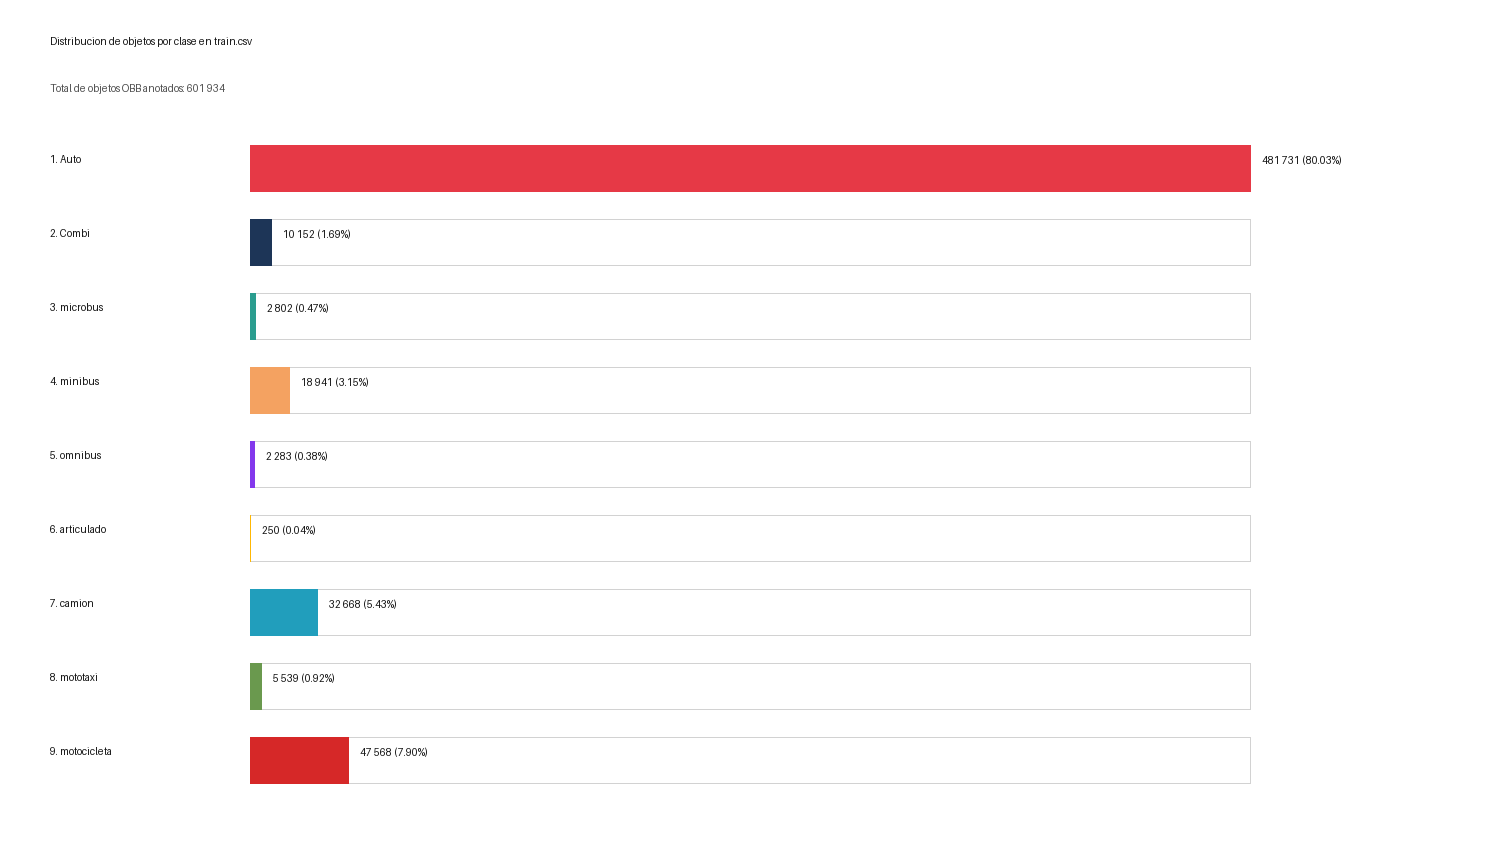
\includegraphics[width=0.95\textwidth]{latex_report/src/fig/dataset_class_distribution.png}
  \caption{Distribuci{\'o}n de objetos anotados por clase vehicular en el conjunto de entrenamiento.}
  \label{fig:dataset_class_distribution}
\end{figure*}

La estructura temporal tambi{\'e}n es importante para el dise{\~n}o experimental. En entrenamiento se identificaron 1 088 clips anonimizados, con un m{\'i}nimo de 18 frames por clip, una media de 49.87, una mediana de 50 y un m{\'a}ximo de 50. En prueba se identificaron 473 clips, con un m{\'i}nimo de 23 frames, media de 49.85, mediana de 50 y m{\'a}ximo de 50. Esta organizaci{\'o}n indica que muchos frames son temporalmente cercanos; por ello, la partici{\'o}n de validaci{\'o}n debe realizarse por clips completos y no por frames individuales, ya que mezclar frames consecutivos del mismo clip entre entrenamiento y validaci{\'o}n podr{\'i}a sobreestimar el rendimiento del modelo.

\begin{figure}[htbp]
  \centering
  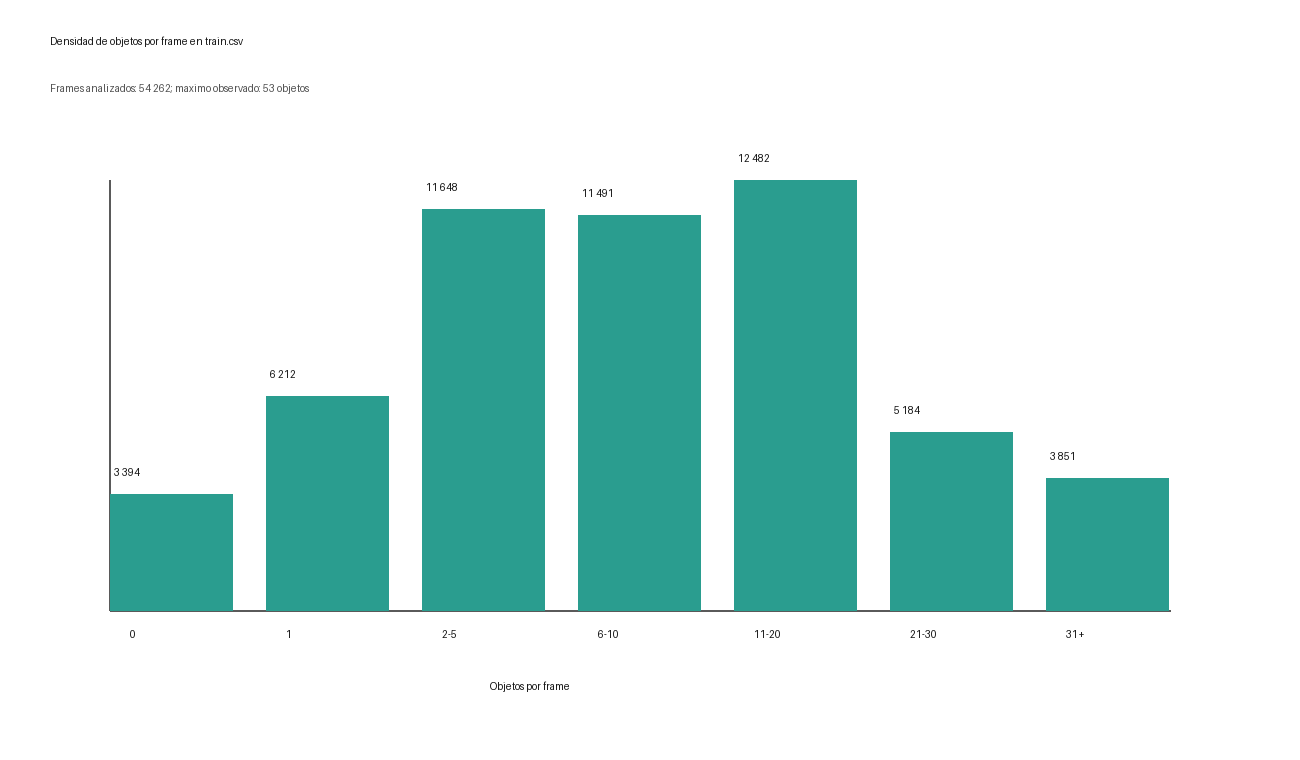
\includegraphics[width=\columnwidth]{latex_report/src/fig/dataset_objects_per_frame.png}
  \caption{Distribuci{\'o}n de densidad de objetos por frame en \texttt{train.csv}.}
  \label{fig:dataset_objects_per_frame}
\end{figure}

La revisi{\'o}n visual confirma que las anotaciones corresponden a cajas orientadas sobre veh{\'i}culos observados desde una perspectiva superior. La Fig.~\ref{fig:dataset_obb_sample} muestra un frame de una intersecci{\'o}n urbana con autos, combi, cami{\'o}n, minibus y motocicleta, donde las cajas siguen la orientaci{\'o}n real de cada veh{\'i}culo. Este ejemplo ilustra por qu{\'e} una representaci{\'o}n horizontal ser{\'i}a insuficiente: algunos veh{\'i}culos aparecen alineados con carriles horizontales, otros con carriles verticales o maniobras de giro, y otros se ubican en zonas de borde o con tama{\~n}os reducidos. En consecuencia, el dataset exige conservar la geometr{\'i}a orientada durante la conversi{\'o}n y el entrenamiento.

\begin{figure*}[htbp]
  \centering
  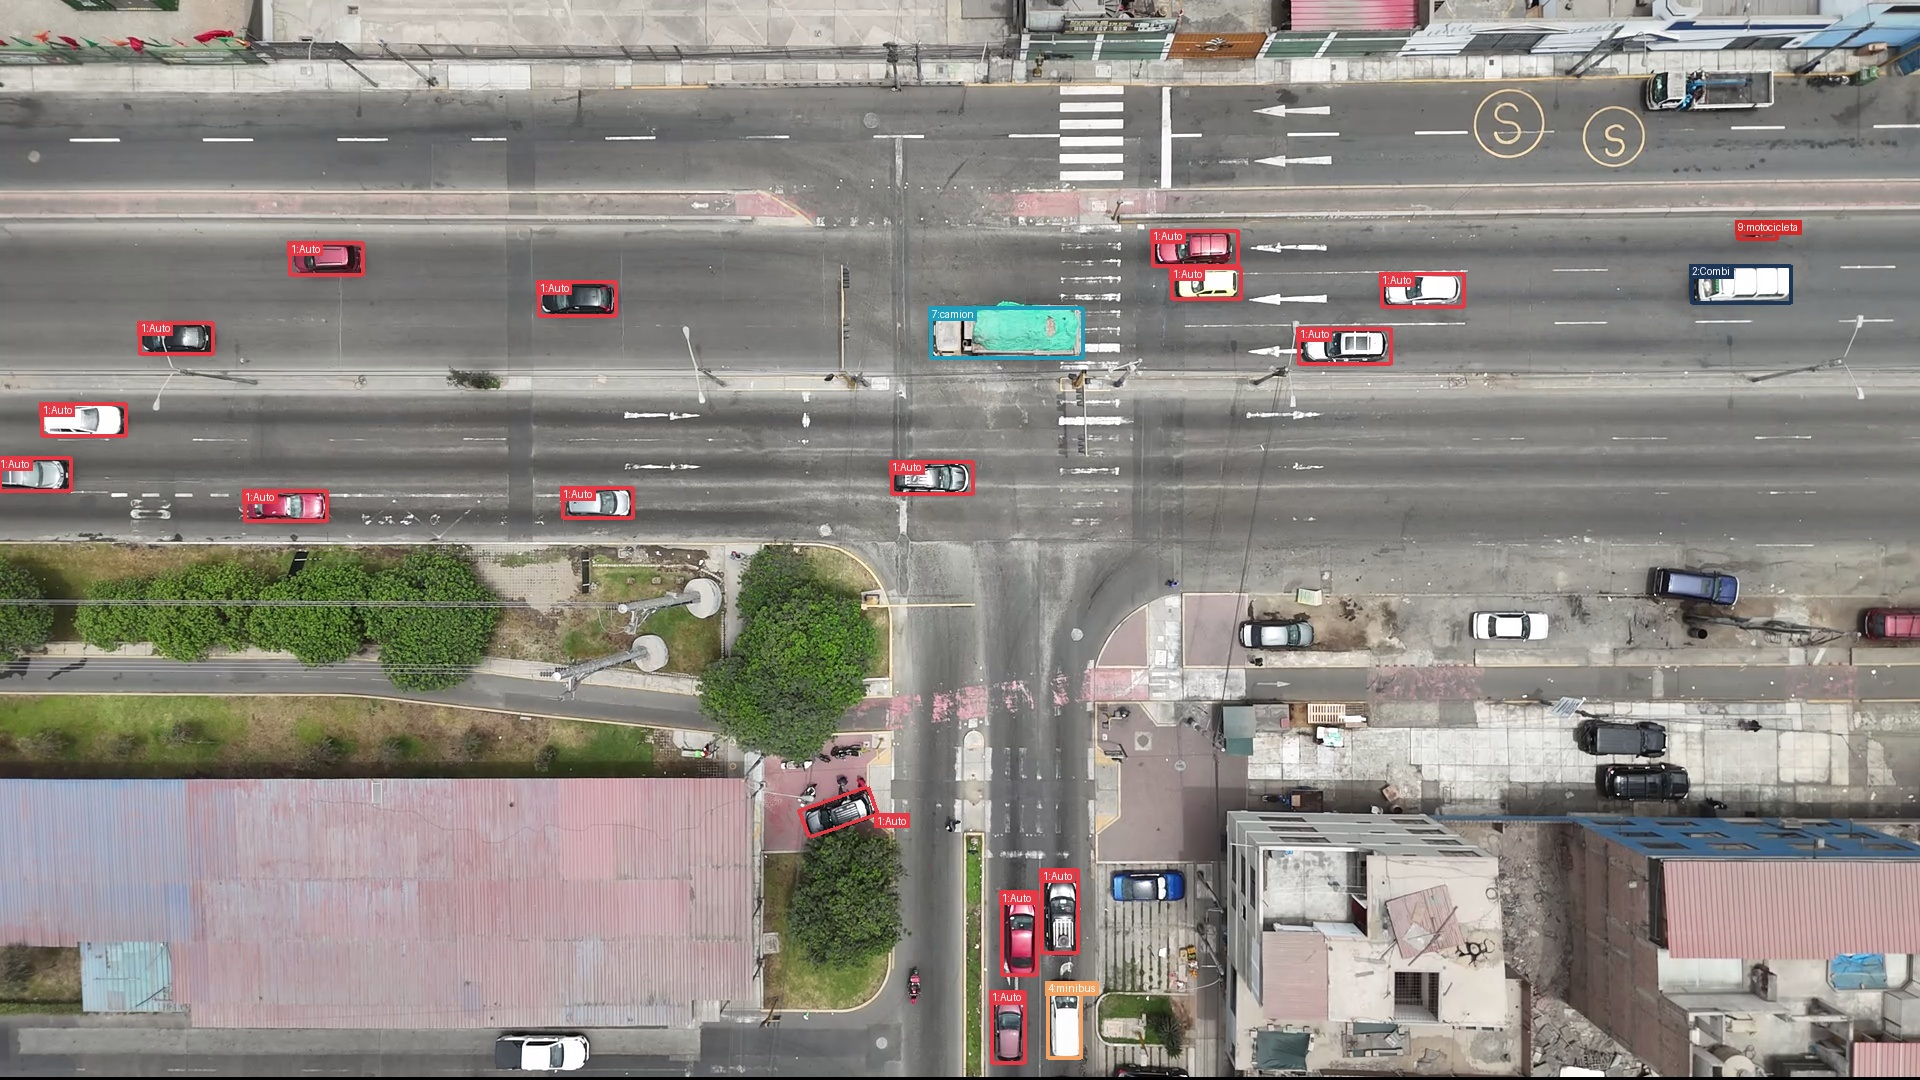
\includegraphics[width=0.95\textwidth]{latex_report/src/fig/dataset_obb_sample.jpg}
  \caption{Ejemplo de frame del conjunto \texttt{muestra\_300/} con anotaciones OBB dibujadas sobre veh{\'i}culos.}
  \label{fig:dataset_obb_sample}
\end{figure*}

En t{\'e}rminos metodol{\'o}gicos, el dataset debe tratarse como un conjunto de frames derivados de clips, no como im{\'a}genes independientes sin relaci{\'o}n temporal. La conversi{\'o}n a un formato compatible con YOLO OBB debe mapear las clases oficiales de 1--9 a clases internas 0--8 y revertir ese mapeo al generar la entrega final. Los frames con \texttt{Target == none} deben mantenerse como im{\'a}genes negativas, porque aportan informaci{\'o}n sobre ausencia de veh{\'i}culos anotados y ayudan a controlar falsos positivos. Finalmente, debido al desbalance de clases y a la evaluaci{\'o}n macro, el an{\'a}lisis del modelo no debe limitarse a la precisi{\'o}n global, sino reportar el comportamiento por clase, especialmente en \texttt{articulado}, \texttt{omnibus}, \texttt{microbus}, \texttt{mototaxi} y \texttt{combi}.
